
% LaTeX Beamer file automatically generated from DocOnce
% https://github.com/hplgit/doconce

%-------------------- begin beamer-specific preamble ----------------------

\documentclass{beamer}

\usetheme{blue_plain}
\usecolortheme{default}

% turn off the almost invisible, yet disturbing, navigation symbols:
\setbeamertemplate{navigation symbols}{}

% Examples on customization:
%\usecolortheme[named=RawSienna]{structure}
%\usetheme[height=7mm]{Rochester}
%\setbeamerfont{frametitle}{family=\rmfamily,shape=\itshape}
%\setbeamertemplate{items}[ball]
%\setbeamertemplate{blocks}[rounded][shadow=true]
%\useoutertheme{infolines}
%
%\usefonttheme{}
%\useinntertheme{}
%
%\setbeameroption{show notes}
%\setbeameroption{show notes on second screen=right}

% fine for B/W printing:
%\usecolortheme{seahorse}

\usepackage{pgf}
\usepackage{graphicx}
\usepackage{epsfig}
\usepackage{relsize}
\documentclass[tikz]{standalone}
\usetikzlibrary{arrows,decorations.pathreplacing}
\usepackage{fancybox}  % make sure fancybox is loaded before fancyvrb
\usepackage{fancyvrb}
%\usepackage{minted} % requires pygments and latex -shell-escape filename
%\usepackage{anslistings}
%\usepackage{listingsutf8}

\usepackage{amsmath,amssymb,bm}
%\usepackage[latin1]{inputenc}
\usepackage[T1]{fontenc}
\usepackage[utf8]{inputenc}
\usepackage{colortbl}
\usepackage[english]{babel}
\usepackage{tikz}
\usetikzlibrary{positioning}
\usetikzlibrary{fit}
\usetikzlibrary{backgrounds}
\usetikzlibrary{calc}
\usetikzlibrary{shapes}
\usetikzlibrary{mindmap}
\usetikzlibrary{decorations.text}
%\pgfplotsset{compat=1.7}
\usepackage{multirow}

\usepackage{framed}
% Use some nice templates
\beamertemplatetransparentcovereddynamic
\usepackage{graphicx}
\graphicspath{{figures/}}
% --- begin table of contents based on sections ---
% Delete this, if you do not want the table of contents to pop up at
% the beginning of each section:
% (Only section headings can enter the table of contents in Beamer
% slides generated from DocOnce source, while subsections are used
% for the title in ordinary slides.)
\AtBeginSection[]
{
  \begin{frame}<beamer>[plain]
  \frametitle{}
  %\frametitle{Outline}
  \tableofcontents[currentsection]
  \end{frame}
}
% --- end table of contents based on sections ---

% If you wish to uncover everything in a step-wise fashion, uncomment
% the following command:

%\beamerdefaultoverlayspecification{<+->}

\newcommand{\shortinlinecomment}[3]{\note{\textbf{#1}: #2}}
\newcommand{\longinlinecomment}[3]{\shortinlinecomment{#1}{#2}{#3}}
\usepackage{xcolor}

\newcommand{\highlight}[1]{%
  \colorbox{red!50}{$\displaystyle#1$}}

\definecolor{linkcolor}{rgb}{0,0,0.4}
\hypersetup{
    colorlinks=true,
    linkcolor=linkcolor,
    urlcolor=linkcolor,
    pdfmenubar=true,
    pdftoolbar=true,
    bookmarksdepth=3
    }
\setlength{\parskip}{0pt}  % {1em}

\newenvironment{doconceexercise}{}{}
\newcounter{doconceexercisecounter}
\newenvironment{doconce:movie}{}{}
\newcounter{doconce:movie:counter}

\newcommand{\subex}[1]{\noindent\textbf{#1}}  % for subexercises: a), b), etc

%-------------------- end beamer-specific preamble ----------------------

% Add user's preamble
% insert custom LaTeX commands...

\raggedbottom
\makeindex
\tikzset{
   invisible/.style={opacity=0},
   visible on/.style={alt=#1{}{invisible}},
   alt/.code args={<#1>#2#3}{%
      \alt<#1>{\pgfkeysalso{#2}}{\pgfkeysalso{#3}} % \pgfkeysalso doesn't change the path
   },
}
%-------------------- end preamble ----------------------

\begin{document}


% matching end for #ifdef PREAMBLE
% #endif
% ------------------- main content ----------------------
% ----------------- title -------------------------

\title{Gender differences in an endogenous timing conflict game}

% ----------------- author(s) -------------------------

\author{Philip Grossman\inst{1} \and Youngseok Park\inst{2}\and Jean Paul Rabanal\inst{1} \and Olga Rud\inst{3} }
\institute{\inst{1} Monash University \inst{2} Korea Institute for International Economic Policy \inst{3} RMIT University}
% ----------------- end author(s) -------------------------

\date{\today
}


\begin{frame}[plain,fragile]
\titlepage
\end{frame}


\frame
{
\frametitle{about my (and coauthors') current work }
\begin{itemize}
\item exploration/exploitation in continuous games

\begin{figure}[here]
\begin{center}
\includegraphics[scale=.30]{inoutex.png}
\label{fig:inoutscree}
\par\end{center}
\end{figure} 
\end{itemize}

}

\frame
{
\frametitle{Competition and performance}
\begin{itemize}
\item Do better forecasters improve convergence in a Learning to Forecast Experiment? 

\item Does competition distort incentives of intermediaries? 
\end{itemize}
}

\frame
{
\frametitle{ETFs}
\begin{itemize}
\item the role of exchange traded funds (ETFs) in financial markets

\begin{figure}[here]
\begin{center}
\includegraphics[scale=.25]{etfs_screen.png}
\label{fig:etf}
\par\end{center}
\end{figure} 


\end{itemize}
}


\frame
{
\frametitle{Motivation}
\begin{itemize}
\item women are willing to volunteer more often than men when their incentives align with the social welfare (Babcock et al., 2017)

\item a socially optimal choice could be risky.

\end{itemize}
}

\frame
{
\frametitle{Summary}
\begin{itemize}
\item The fear of choosing the socially optimal appears in Baliga and Sj\"ostr\"om (2004, hereafter BS04).

\item BS04 is a simultaneous-move game. 

\item  we extend to 
\begin{itemize}
    \item exogenous sequential game
    \item endogenous timing (either one-shot or sequential)
\end{itemize}

\item gender differences appear in the endogenous timing. men play the risky payoff dominant strategy more often than women. 

\end{itemize}
}
 
 \frame
{
\frametitle{BS04 conflict game (CGO)}
two players, two actions: H \& D. 

\begin{equation}
\begin{pmatrix}
x_i & 10+x_i \\
5 & 100
\label{t:payoff}
\end{pmatrix},
\end{equation}

where $x_i \sim U[0,100]$

A player with a payout lower than $x_i\leq\hat{x}_{_{CGO}}$ will play $D$ and $H$ otherwise

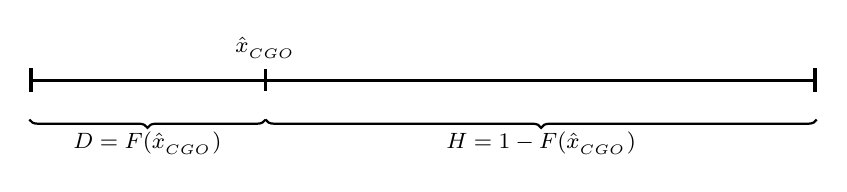
\begin{tikzpicture}[y=1cm, x=1cm, thick, font=\footnotesize]    
% axis
\draw[line width=1.2pt, |-|, >=latex'](0,0) -- coordinate (x axis) (10,0);       
\draw (3,-4pt) coordinate (t_k)          -- (3,4pt) node[anchor=south] {$\hat{x}_{_{CGO}}$};
% curly braces
\draw[decorate,decoration={brace,amplitude=3pt,mirror}] 
    (0,-0.5) coordinate (t_k_unten) -- (3,-0.5) coordinate (t_k_opt_unten); 
\node at (1.5,-0.8){$D=F(\hat{x}_{_{CGO}})$};
\draw[decorate,decoration={brace,amplitude=3pt,mirror}] 
    (3,-0.5) coordinate (t_k_unten) -- (10,-0.5) coordinate (t_k_opt_unten); 
\node at (6.5,-0.8){$H=1-F(\hat{x}_{_{CGO}})$};
\end{tikzpicture}

\item We can solve for the cutoff point:
\begin{equation}
\hat{x}_{_{CGO}}= 5 + \highlight{(85)} F(\hat{x}_{_{CGO}}). \label{eq:cgo}
\end{equation}
}

\frame
{
\frametitle{A sequential game (CGS) can improve social welfare}
\begin{itemize}
\item \emph{strategic complements} game: first mover that sets the stage 
\item If first player plays $D$, there is an incentive for the second player to follow suit 

\item Sequential game can help improve social welfare!

\item a unique PBNE where the first mover follows the cutoff strategy 
\begin{equation}
\sigma_i(x_i)=D \quad \text{if} \ \ x_i\leq \hat{x}_{_{CGS}} \equiv 100-10. 
\end{equation}

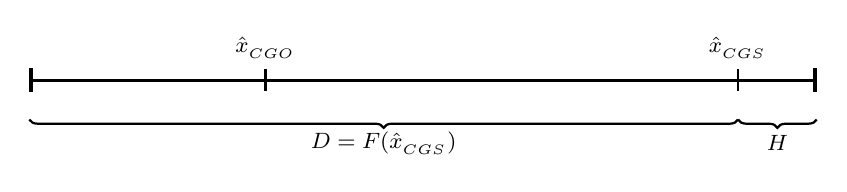
\begin{tikzpicture}[y=1cm, x=1cm, thick, font=\footnotesize]    
% axis
\draw[line width=1.2pt, |-|, >=latex'](0,0) -- coordinate (x axis) (10,0);       
\draw (3,-4pt) coordinate (t_k)          -- (3,4pt) node[anchor=south] {$\hat{x}_{_{CGO}}$};
\draw (9,-4pt) coordinate (t_k)          -- (9,4pt) node[anchor=south] {$\hat{x}_{_{CGS}}$};
% curly braces
\draw[decorate,decoration={brace,amplitude=3pt,mirror}] 
    (0,-0.5) coordinate (t_k_unten) -- (9,-0.5) coordinate (t_k_opt_unten); 
\node at (4.5,-0.8){$D=F(\hat{x}_{_{CGS}})$};
\draw[decorate,decoration={brace,amplitude=3pt,mirror}] 
    (9.0,-0.5) coordinate (t_k_unten) -- (10,-0.5) coordinate (t_k_opt_unten); 
\node at (9.5,-0.8){$H$};
\end{tikzpicture}
\end{itemize}
}



\frame
{
\frametitle{Endogenous order of play (CGE)}
\begin{itemize}
\item The game proceeds as follows:
\begin{itemize}
\item \textit{Stage 0:} Each player $i$ selects a cutoff strategy, indicating a set of values where $\sigma_i(x_i)=H$, and then observes own type $x_i$, but not the other player's type $x_j$ where $j\neq i$.

\item  \textit{Stage 1:} Both players simultaneously select the period in which to play the game $t=1,2$. 

\item \textit{Stage 2:} The conflict game is played by the move structure determined in Stage 1. The commitment to the cutoff strategy is not binding for the player $i$ if and only if $t_i=2$ and $t_j=1$. 
\end{itemize}
\item coordination issues: the BNE is either $\hat{x}_{_{CGO}}$ or $\hat{x}_{_{CGS}}$
\end{itemize}

 }
 
 \frame	
{
\frametitle{Cutoff User-Interface }
\begin{figure}[here]
\begin{center}
\includegraphics[scale=.35]{cutoffen.png}
\label{fig:usercutoff}
\par\end{center}
\end{figure} 
}

  \frame	
{
\frametitle{Timeline}
 \begin{table}[ht]
 \footnotesize
\begin{center}
\begin{tabular}{l|>{\columncolor[HTML]{FFCE93}\color{blue}}m{2.5cm}|m{3.5cm}|m{3cm}}
  Step & CGO & CGS & CGE\\
  \hline 
I & Cutoff & Cutoff & Cutoff \\
\hline
II& $x_i$ is revealed; H if $\mtext{cutoff}\leq x_i$ & $x_i$ is revealed; H if $\mtext{cutoff}\leq x_i$ for 1st mover (randomly chosen)
& $x_i$ is revealed; choose $t=\{1,2\}$ with action commitment defined according to $\mtext{cutoff}$\\
\hline
III & - & 2nd mover picks \textbf{s} & 2nd mover ($t=2$) picks \textbf{s} if other chose $t=1$. Otherwise, the game is a oneshot.

\end{tabular}
\end{center}
\caption{Timeline for each treatment}
\label{table:time}
\end{table}
 }
 
   \frame	
{
\frametitle{Timeline}
 \begin{table}[ht]
 \footnotesize
\begin{center}
\begin{tabular}{l|m{2.5cm}|>{\columncolor[HTML]{FFCE93}\color{blue}}m{3.5cm}|m{3cm}}
  Step & CGO & CGS & CGE\\
  \hline 
I & Cutoff & Cutoff & Cutoff \\
\hline
II& $x_i$ is revealed; H if $\mtext{cutoff}\leq x_i$ & $x_i$ is revealed; H if $\mtext{cutoff}\leq x_i$ for 1st mover (randomly chosen)
& $x_i$ is revealed; choose $t=\{1,2\}$ with action commitment defined according to $\mtext{cutoff}$\\
\hline
III & - & 2nd mover picks \textbf{s} & 2nd mover ($t=2$) picks \textbf{s} if other chose $t=1$. Otherwise, the game is a oneshot.

\end{tabular}
\end{center}
\caption{Timeline for each treatment}
\label{table:time2}
\end{table}
 }
    \frame	
{
\frametitle{Timeline}
 \begin{table}[ht]
 \footnotesize
\begin{center}
\begin{tabular}{l|m{2.5cm}|m{3.5cm}|>{\columncolor[HTML]{FFCE93}\color{blue}}m{3cm}}
  Step & CGO & CGS & CGE\\
  \hline 
I & Cutoff & Cutoff & Cutoff \\
\hline
II& $x_i$ is revealed; H if $\mtext{cutoff}\leq x_i$ & $x_i$ is revealed; H if $\mtext{cutoff}\leq x_i$ for 1st mover (randomly chosen)
& $x_i$ is revealed; choose $t=\{1,2\}$ with action commitment defined according to $\mtext{cutoff}$\\
\hline
III & - & 2nd mover picks \textbf{s} & 2nd mover ($t=2$) picks \textbf{s} if other chose $t=1$. Otherwise, the game is a oneshot.

\end{tabular}
\end{center}
\caption{Timeline for each treatment}
\label{table:time3}
\end{table}
 }
 
 \frame
{
\frametitle{Procedures}
\begin{itemize}
\item Subjects recruited from Universidad del Rosario, Bogota, Colombia (ORSEE)
\item Show-up fee: COL 10K $\approx$ \$ 3.3
\item A between design, veiled gender, perfect stranger matching
\item 3 treatments: CGO, GGS and GGE
\item Each session: 
\begin{itemize}
    \item two silos
    \item 12 Ss in each silo 
    \item (almost) balance gender composition within silo
    \item each silo runs a different treatment 
\end{itemize}
\item oTree user-interface 

\end{itemize}
}


\frame
{
\frametitle{Summary of results (pooled data)}
\begin{center}
\begin{figure}[ht]
\centering{}%
\includegraphics[scale=0.5]{jointcut.pdf}%
%\caption{CDF of $x$ by subject in CM and DM. Each observation is based on the median subject choice for periods 26-50. The vertical lines represent the predicted equilibrium under DM and CM. }
\label{fig:jointcut}
\end{figure}
\par\end{center}
}



\frame
{
\frametitle{CGE (pooled data)}
\begin{center}
\begin{figure}[ht]
\centering{}%
\includegraphics[scale=0.5]{countgendermoveplay.pdf}%
%\caption{CDF of $x$ by subject in CM and DM. Each observation is based on the median subject choice for periods 26-50. The vertical lines represent the predicted equilibrium under DM and CM. }
\label{fig:jointcut}
\end{figure}
\par\end{center}
}




\frame	
{
\frametitle{CGE (pooled data)}
\begin{table}[ht]
\centering
\begin{tabular}{l|c>{\columncolor[HTML]{FFCE93}\color{blue}}cc}
    & one-shot $t=1$  & seq. & one-shot $t=2$\\
    \hline
  HH    &    2.31 &17.59  &      3.24\\
  HD    &    6.48 & 3.70 &      15.28\\
  DD     &   5.09 &34.72&       11.57
\end{tabular}
\label{table1}
\caption{CGE. Frequency of cells and timing (\%) }

\end{table}
}

\frame
{
\frametitle{Subject data}
\begin{center}
\begin{figure}[ht]
\centering{}%
\includegraphics[scale=0.5]{cdfcutoff.pdf}%
%\caption{CDF of $x$ by subject in CM and DM. Each observation is based on the median subject choice for periods 26-50. The vertical lines represent the predicted equilibrium under DM and CM. }
\label{fig:allcdfsubj}
\end{figure}
\par\end{center}
}

\frame
{
\frametitle{Subject data - women}
\begin{center}
\begin{figure}[ht]
\centering{}%
\includegraphics[scale=0.5]{cdfcutoffgender_female.pdf}%
%\caption{CDF of $x$ by subject in CM and DM. Each observation is based on the median subject choice for periods 26-50. The vertical lines represent the predicted equilibrium under DM and CM. }
\label{fig:fecdfsubj}
\end{figure}
\par\end{center}
}

\frame
{
\frametitle{Subject data - men}
\begin{center}
\begin{figure}[ht]
\centering{}%
\includegraphics[scale=0.5]{cdfcutoffgender_male.pdf}%
%\caption{CDF of $x$ by subject in CM and DM. Each observation is based on the median subject choice for periods 26-50. The vertical lines represent the predicted equilibrium under DM and CM. }
\label{fig:fecdfsubj}
\end{figure}
\par\end{center}
}

\frame
{
\frametitle{Subject data - CGO}
\begin{center}
\begin{figure}[ht]
\centering{}%
\includegraphics[scale=0.5]{cdfcutoffgender_o.pdf}%
%\caption{CDF of $x$ by subject in CM and DM. Each observation is based on the median subject choice for periods 26-50. The vertical lines represent the predicted equilibrium under DM and CM. }
\label{fig:onecdfsubj}
\end{figure}
\par\end{center}
}

\frame
{
\frametitle{Subject data - CGS}
\begin{center}
\begin{figure}[ht]
\centering{}%
\includegraphics[scale=0.5]{cdfcutoffgender_s.pdf}%
%\caption{CDF of $x$ by subject in CM and DM. Each observation is based on the median subject choice for periods 26-50. The vertical lines represent the predicted equilibrium under DM and CM. }
\label{fig:sscdfsubj}
\end{figure}
\par\end{center}
}

\frame
{
\frametitle{Subject data - CGE}
\begin{center}
\begin{figure}[ht]
\centering{}%
\includegraphics[scale=0.5]{cdfcutoffgender_e1.pdf}%
%\caption{CDF of $x$ by subject in CM and DM. Each observation is based on the median subject choice for periods 26-50. The vertical lines represent the predicted equilibrium under DM and CM. }
\label{fig:eecdfsubj}
\end{figure}
\par\end{center}
}


\frame	
{
\frametitle{DD frequencies}
\begin{table}[!t]
\centering
\begin{tabular}{lcccccc>{\columncolor[HTML]{FFCE93}\color{blue}}c}

Treatment & Group 1 & G2  & G3 & G4 & G5 & G6 & Mean\\
  \hline
  CGO &  19.44 & 19.44&  27.78 & 27.78 & 36.11 & 52.78 & 30.56 \\
  CGS & 30.56 & 47.22&  50.00 & 52.78 & 55.56 & 61.11 & 49.53\\
  GGE & 33.44 & 38.49 & 44.44 & 58.55 & 63.89 & 69.44 & 51.39 \\
  \hline

\end{tabular}
\caption{Frequency (percentage) of cell DD played in sessions }
\label{table:dd}
\end{table}
}




\frame
{
\frametitle{Conclusion}
\begin{itemize}
\item Sequential move improves social welfare 
\item Strategic uncertainty about the timing of the game deters women from playing $D$
\end{itemize}
}


\frame
{
\frametitle{Freq. of H $<$ NE [CGO]}

\begin{itemize}

\item Evdokimov and Garfagnini (2018) find that Freq. of H$\approx .36<$ BNE of .5.

\item Mean-matching may help figure out the distribution of types.

\item In games of complete information, pair vs. mean matching does not seem to matter; not clear in the case of incomplete info. 

\end{itemize}

}

 \frame
{
\frametitle{Freq. of H $>$ NE [CGS] }
\begin{itemize}

\item Heggedal et al (2018) on Farrell and Saloner (1985)

\item Two players, two actions in two periods: I \& N, where $I$ is irreversible. $0<\alpha<1$ and $x \sim U\in[0,10]$
\end{itemize}

\begin{equation}
\begin{pmatrix}
x_i+2 & \alpha \cdot x_i \\
5 & 7
\label{t:payoff}
\end{pmatrix},
\end{equation}
}



\frame
{
\frametitle{Risk of failure}
\begin{itemize}

\item D treatment, $\alpha=1$ while N treatment $\alpha=.5$
\item Risk aversion deters players to commit. 
\end{itemize}

\begin{center}
\begin{figure}[ht]
\centering{}%
\includegraphics[scale=0.3]{fsexp.png}%

\label{fig:fs}
\end{figure}
\par\end{center}
}




\end{document}

